\chapter{Um Motor de Busca Paralelo com STM}

\newcommand{\bigO}[1]{\ensuremath{\operatorname{O}\bigl(#1\bigr)}}

Para entender melhor quais são as diferenças na prática entre os modelos de STM de Clojure e Haskell, foi escolhido como objeto de estudo a implementação de um software não trivial em ambas as linguagens. Trata-se de um motor de busca paralelo para arquivos textuais. Esse problema foi extraído do trabalho de Pankratius e Adi-Tabatabai \cite{pankratius2011study} onde ele é utilizado para comparar a utilização de sincronização baseada em \emph{locks} com a utilização de memória transacional. Nesse experimento, um grupo de alunos de pós-graduação foi dividido em duplas, onde parte das duplas teve que desenvolver o motor de busca utilizando \emph{locks} e outra parte utilizando memória transacional, ambos com a linguagem C++.

Na primeira parte deste capítulo o problema será especificado. Em seguida será descrito em detalhes como a solução do problema foi modelada e implementada nas duas linguagens. E por fim, será levantado as principais diferenças entre as duas implementações.

\section{Especificação}

O motor de busca deve atender aos seguintes requisitos: \cite{pankratius2011study}

\textbf{Indexação}. O motor de busca deve funcionar apenas para arquivos texto e deve realizar a pesquisa em arquivos que estejam em um diretório pré-definido (passado como argumento pela linha de comando) e em todos os seus subdiretórios. Não é necessário que o índice persista em disco. Diferentes estratégias para criação de índices podem ser utilizadas. Toda sequência de caracteres não-alfanuméricos é tratada como separadora de palavras. Diferenças entre letras maiúsculas e minúsculas e hifens são ignorados. Um indicador de progresso para indexação deve mostrar a quantidade de \emph{bytes} e arquivos processados até então, palavras encontradas até então e a quantidade de palavras no índice. A quantidade de \emph{threads} de indexação também deve ser configurável via parâmetro de linha de comando.

\textbf{Busca}. Deve ser possível processar consultas enquanto a indexação ainda está em progresso, mas não é necessário que mais de uma consulta seja executada ao mesmo tempo em paralelo. Fica a cargo do desenvolvedor decidir se paraleliza cada consulta e a quantidade de \emph{threads} que devem ser utilizadas nesse processo. Além disso, a busca deve permitir diferentes tipos de consultas:
\begin{compactenum}
  \item Consultas por passagens de texto coerentes (exemplo, "this is a text");
  \item Consultas com caracteres coringa no começo ou fim de uma palavra (exemplo, "hou*" ou "*pa");
  \item Consultas que contenham uma série de palavras representando uma operação AND (exemplo, "tree house garden");
  \item Consultas com exclusão de palavras (exemplo, "-fruit").
\end{compactenum}

\textbf{Saída}. A saída padrão do programa consiste na quantidade total de arquivos que os critérios de busca são verdadeiros, o tempo de consulta e a listagem dos nomes dos 50 primeiros arquivos ordenados segundo os seguintes critérios:
\begin{compactenum}
  \item Decrescentemente pela quantidade de ocorrências de todos os critérios consultados;
  \item Lexicograficamente pelo nome do arquivo.
\end{compactenum}

Pode-se assumir que durante a execução do programa nenhum arquivo envolvido na busca será alterado nem outros arquivos serão adicionados ou removidos aos diretórios envolvidos na busca.

\section{Versão sequencial}

Inicialmente foi necessário implementar uma versão sequencial do problema proposto para entender melhor o domínio o qual o problema faz parte e também para refletir sobre as estruturas de dados que poderiam ser utilizadas. Essa primeira versão foi escrita em Haskell. Também foi implementada uma tradução dessa versão, em Clojure, com propósito de aprender a linguagem, já que o autor ainda não tinha tido contato com essa linguagem nem com nenhum outro dialeto de Lisp.

\subsection{Índice}

O primeiro passo do desenvolvimento foi decidir qual estrutura de dados seria utilizada para armazenar o índice de palavras. O principal objetivo do índice é prover uma estrutura que associe cada termo presente na base de documentos (o vocabulário) à suas ocorrências nos documentos indexados.

Para esse trabalho foi escolhida uma estrutura bastante utilizada em recuperação de documentos chamada de índices invertidos. Esse tipo de estrutura associa cada palavra  do vocabulário à uma lista de documentos nos quais essa palavra está presente. Existem dois tipos de índices invertidos: os índices invertidos à nível de registro e os índices invertidos à nível de palavra \cite{baeza1999modern}. A diferença entre eles é que o primeiro armazena apenas informação sobre quais documentos a palavra pertence, enquanto o segundo guarda também outras informações como as posições que a palavra ocorre nos documentos. Para realizar as consultas especificadas pelo problema foi necessário utilizar índices invertidos à nível de palavra.

A escolha por utilizar índices invertidos se baseou no fato de ser uma estrutura simples que poderia ser representada de maneira fácil e eficiente em ambas a linguagens utilizando as estruturas de dados providas pelas bibliotecas padrão. Adicionalmente, com a intenção de melhorar um pouco a performance das consultas, foram utilizados um conjunto de índices invertidos ao invés de apenas um único índice global, onde cada índice invertido armazena apenas palavras iniciadas com uma determinada letra. Dessa forma, tem-se um índice invertido para cada caracter possível, totalizando 35 índices. A Figura \ref{fig:indice} contém uma representação gráfica do índice. No restante desse trabalho a palavra índice será utilizada para denotar a estrutura descrita neste parágrafo e representada graficamente na Figura \ref{fig:indice}.

\begin{figure}[h]
 \centering
 \def\svgwidth{0.6\columnwidth}
 \input{estrutura-indice.pdf_tex}
 \caption{Representação do índice}
 \label{fig:indice}
\end{figure}


Em Haskell o índice foi representado utilizando-se um tipo \verb|Array| (do módulo \verb|Data.Array|) para armazenar todos os índices invertidos e um \verb|Map| (do módulo \verb|Data.Map|) para cada índice invertido. O \verb|Array| provê acesso \bigO{1} aos seus elementos, enquanto o \verb|Map| provê acesso \bigO{log n} aos seus elementos. Cada mapa é armazenado em uma posição do \emph{array} que corresponde ao valor ASCII do caracter referente à primeira letra das palavras contidas no mapeamento em questão. De maneira análoga, em Clojure, foram utilizados as estruturas \verb|vector| e \verb|hash-map| que provêem a mesma complexidade de acesso aos elementos que as estruturas utilizadas em Haskell.

\subsection{Arquitetura}

A versão sequencial foi dividida em 5 módulos: \verb|Scanner|, \verb|Lexer|, \verb|Index|, \verb|Query| e \verb|Main|.

\begin{figure}[h]
 \centering
 \def\svgwidth{0.5\columnwidth}
 \input{arquitetura-sequencial.pdf_tex}
 \caption{Diagrama da arquitetura dos módulos da versão sequencial}
\end{figure}

\textbf{Scanner}. É responsável por percorrer recursivamente o diretório fornecido pelo usuário e seus subdiretórios em busca de arquivos texto. Esse módulo basicamente recebe um caminho como parâmetro e retorna o caminho de todos os arquivos texto achados.

\textbf{Lexer}. É responsável por processar o texto lido de um documento. Primeiramente acontece o pré-processamento do texto, que é recebido como uma \verb|string| única, para remover caracteres não-alfanuméricos, uniformizar a capitalização e quebrar a \verb|string| de entrada em uma lista de \verb|string|s onde cada uma representa uma palavra. Em seguida, transforma essa lista de palavras em um mapeamento onde cada palavra é associada a um conjunto de números que representam as posições que essa palavra aparece no documento. Essa estrutura é chamada de lista de ocorrências.

\textbf{Index}. É responsável por abstrair o acesso ao índice. Neste módulo existem funções para criar um índice, inserir um documento (uma lista de ocorrências) no índice e buscar um termo no índice. Esse módulo é importante pois ele faz com que os demais módulos não precisem ter conhecimento da estrutura interna do índice. Isso faz com que seja possível mudar a estrutura de dados que é utilizada pelo índice sem que o restante do programa precise ser modificado (desde que a API do módulo seja mantida). Essa característica mostra que é possível se alcançar uma modularização semelhante às linguagens orientadas à objeto em uma linguagem funcional utilizando apenas estruturas de dados imutáveis.

\textbf{Query}. É responsável pela construção e execução de consultas. Esse módulos tem funções para realizar o \emph{parsing} da consulta fornecida pelo usuário e para executar uma dada consulta.

\textbf{Main}. É o ponto de entrada do programa. Ele que recebe e faz o \emph{parsing} dos argumentos fornecidos pelo usuário, chama as funções de outros módulos para obter os documentos, processá-los, e inserí-los no índice. Em seguida chama funções do módulo \verb|Query| para realizar a consulta e, por fim, imprime o resultado final com o ordenamento e a formatação correta para o usuário.


\section{Versão paralela}

A versão paralela do motor de busca foi fortemente baseada na versão sequêncial. Tanto a versão paralela escrita em Haskell como a escrita em Clojure atendem à todos os pontos listados na especificação do problema com exceção dos tipos de consulta suportados. Apenas as consultas por passagens de texto coerentes foram implementadas devido ao tempo reduzido disponível para implementação do problema em duas linguagens distintas. Adicionalmente, embora não fosse um requisito obrigatório, as consultas são executadas de foma paralela em ambas as versões.

\subsection{Índice}

A estrutura do índice em si é a mesma da versão sequencial. Porém, como deve ser possível executar consultas durante o processo de indexação, a utilização do índice teve que ser repensada. A razão para isso é que na versão sequencial é utilizado apenas um índice global que armazena os termos de toda base de documentos. Se na versão paralela essa mesma abordagem fosse utilizada, a paralelização das consultas não melhoraria o desempenho da aplicação pois consultas consecutivas iriam sempre ter resultados cumulativos. Por exemplo, se uma consulta for executada quando apenas 2 documentos foram indexados, um resultado parcial \emph{X} será produzido. Se a mesma consulta for executada novamente no futuro, quando um total de 5 documentos tiverem sido indexados, o resultado produzido será \emph{X + Y}, onde \emph{Y} consiste no resultado da consulta nos 3 novos arquivos que foram indexados. Dessa forma, não se tem ganho na paralelização das consultas.

Para contornar esse problema, existem duas técnicas que podem ser aplicadas para realizar o processamento paralelo de consultas: o particionamento de documentos e o particionamento de termos \cite{buttcher2010information}. As duas abordagens dividem o índice em subíndices por meio de uma \emph{n}-partição por disjunção. Na primeira abordagem cada subíndice contém um subconjunto do conjunto de todos os da base de documentos, enquanto na segunda, cada subíndice contém um subconjunto do conjunto de todos os termos. Para o propósito desse trabalho apenas o particionamento de documentos pode ser utilizado porque o particionamento de termos necessita de um conhecimento prévio da base de documentos.

\begin{figure}[h]
 \centering
 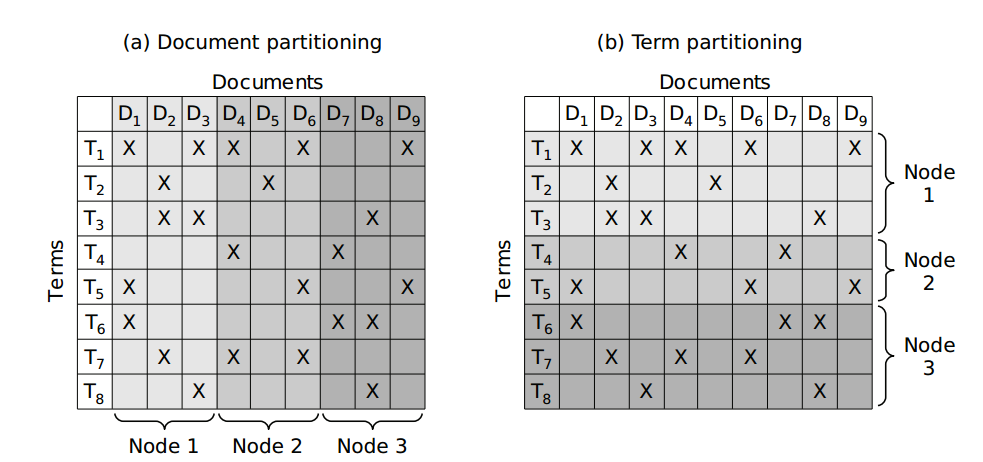
\includegraphics[scale=0.5]{imagens/particionamento-indice.png}
 \caption{Representação das duas abordagens de particionamento de índice}
\end{figure}

Assim, para resolver o problema da consulta durante a indexação são utilizados vários subíndices onde cada um tem um número máximo de documentos que podem ser indexados. Quando um subíndice atinge o número máximo de documentos ele está pronto para ser consultado. Tanto o número máximo de documentos por subíndice quanto a quantidade inicial de subíndices criados podem ser configurados pelo usuário por meio de argumentos de linha de comando.

\subsection{Arquitetura}

Alguns módulos utilizados na versão sequencial foram mantidos sem modificações, como foi o caso do \verb|Lexer|, \verb|Index| e \verb|Query|. Porém, para atender aos requisitos de paralelização, os demais módulos tiveram que ser modificados e outros tiveram que ser criados.

\begin{figure}[h]
 \centering
 \def\svgwidth{0.6\columnwidth}
 \input{arquitetura-paralelo.pdf_tex}
 \caption{Diagrama simplificado de como é feita a comunição entre threads}
\end{figure}

\textbf{Scanner}. Esse módulo teve que ser mudado para que a busca por documentos acontecesse em uma \emph{thread} separada. Assim, a descoberta de arquivos é executada paralelamente ao processamento e a indexação dos documentos. Esse comportamento caracteriza um modelo produtor-consumidor onde o \verb|Scanner| é o produtor, e as \emph{threads} de processamento e indexação são os consumidores. Tanto na versão Clojure como na versão Haskell esse modelo é implementado por meio de um \emph{buffer} compartilhado de capacidade infinita que bloqueia os consumidores que tentam ler do \emph{buffer} vazio até que novos elementos sejam produzidos.

\textbf{Engine}. Esse módulo é responsável pelo orquestramento das \emph{threads} de processamento e indexação de documentos e também das \emph{threads} de consulta. Inicialmente são criadas \emph{n} \emph{threads}\footnote{\emph{n} é fornecido pelo usuário} responsáveis pelo processamento e indexação dos documentos. Cada \emph{thread} executa em \emph{loop} enquanto houverem arquivos para serem processados. Esses arquivos são lidos do \emph{buffer} compartilhado com o \verb|Scanner|. Para cada arquivo que é lido, ele é processado, e em seguida indexado em um dos subíndices disponíveis. Após a indexação, se o subíndice estiver cheio (já tiver completado o número máximo de documentos por subíndice), ele é marcado como pronto e um novo subíndice vazio é adicionado à lista de subíndices disponíveis. Esse é o funcionamento das \emph{threads} de processamento e indexação. Já a parte das consultas funcionam da seguinta forma: sempre que um subíndice é marcado como pronto, uma nova \emph{thread} é criada para cada consulta fornecida pelo usuário. Cada \emph{thread} de consulta vai executar a consulta no subíndice e concatenar o resultado em uma variável transacional que é utilizada para acumular o resultado dessa consulta. Ao final, quando todos os subíndices tiverem sido consultados, cada variável transacional terá o resultado completo de uma consulta.

\textbf{Buffer}. Esse módulo abstrai o acesso aos \emph{buffers} que são compatilhados entre \emph{threads}. Contém funções para criação, adição e remoção de elementos.

\textbf{Logger}. É responsável por gerenciar o indicador de progresso do programa. Ele roda em uma \emph{thread} separada e fica recebendo mensagens de status dos demais módulos informando o progresso. Baseado nesses status as mensagens de indicação de progresso são formatadas e impressas no \emph{console} para o usuário durante a execução do programa.

\textbf{Main}. Como o controle do processamento dos arquivos e das consultas foi delegado ao módulo \verb|Engine|, o \verb|Main| na versão paralela apenas faz o \emph{parsing} dos parâmetros fornecidos pelo usuário e inicia o \verb|Scanner|, o \verb|Engine| e o \verb|Logger|.